\subsection{The Motivation}

Our goal when we integrate a function is to find the amount of `space' between the graph and x-axis (or the Abscissa if you're fancy - but I'll just say x-axis). It's pretty difficult to say how much space an arbitrary curve takes up, but we can work out the area of rectangles very easily - by calculating the {\em base $\times$ height}. Riemann integration takes advantage of this, and defines the integral of a function $f:\R \rightarrow \R$ by first bounding it from above with rectangular functions and finding the smallest of these areas (which is would be an upper bound for the area of the function), then we bound the function from below and find an lower bound, then we hope that these two bounds match up. 

\begin{figure}[H]
\centering
\begin{minipage}{.5\textwidth}
  \centering
  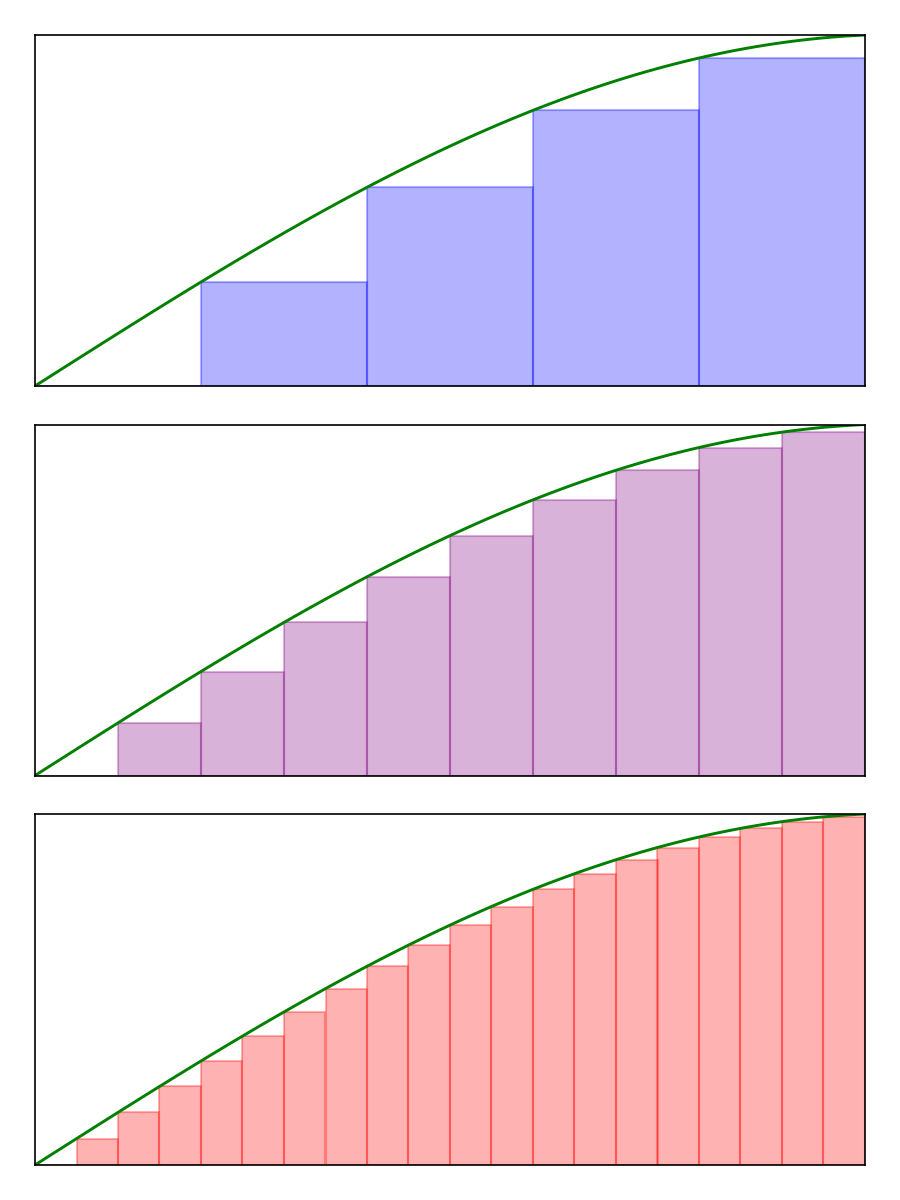
\includegraphics{Code/Area1.png}
  \captionof{figure}{Bounding from Below}
  \label{fig:test1}
\end{minipage}%
\begin{minipage}{.5\textwidth}
  \centering
  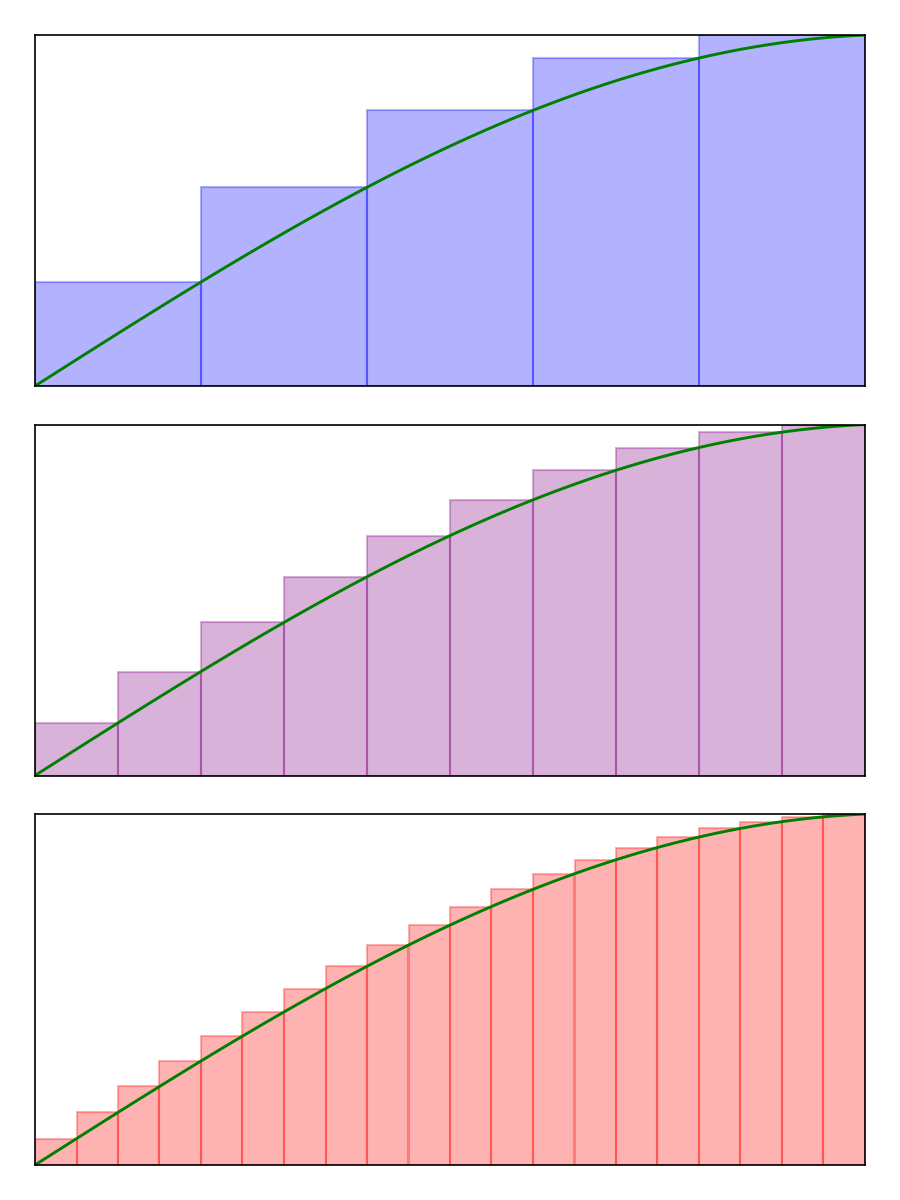
\includegraphics{Code/Area2.png}
  \captionof{figure}{Bounding from Above}
  \label{fig:test1}
\end{minipage}
\end{figure}

If the domain of our function (the `x-axis'), is $\R^2$ instead of just $\R$, we'd actually calculating a volume by finding the `space' between the graph and the axis. Basic Riemann integration doesn't apply to these functions - still, you can think of the `area of a rectangle' (which in $R^2 \rightarrow \R$ would actually be the volume of a cuboid) as being calculated in much the same way; the size of the base (which is now an area, instead of a length) $\times$ the height. With this is mind, lets clear up some of the terms we are going to use:

\begin{description}
\item[\em Lebesgue integration\/] is the method of integration defined above. Just like Riemann Integration, it is used to find the space between the graph of a function and the domain. However, unlike Riemann, the domain can be any set at all. Thinking back to rectangles and cuboids and $base \times height$, if we wanted make sense of what it means for there to be space between the graph and the x-axis, we should be able to make sense of the `size' of parts of the domain, so that we can figure out how big our base is and multiply that by the height$\ldots$
%
\item[\em The Lebesgue Measure\/] seems then like it'd be a way to assign sizes to, or `measure' sets in the domain; but it is not! It's a term used specifically when we give sizes to the subsets of $\R^n$, and those sizes (or `measures') coincided with our usual idea of the size of a set in $\R^n$ - i.e. it is used when we are considering functions $\R^n \supset Y \rightarrow \R$, and in $\R$ the measure (length) of the interval $[1, 0]$ is 1, in $\R^2$ the measure (area) of the rectangle $[1, 0] \times [1, 0]$ is 1, in $\R^3$ the measure (volume) of the cube $[1, 0] \times [1, 0] \times [1, 0]$ is 1$\ldots$ etc. 
%
\item[\bf \em The Lebesgue Integral\/] is what we get when we do Lebesgue Integration on a set with the Lebesgue Measure on it. i.e. it's the integral of normal functions $\R^n \supset Y \rightarrow \R$. This is the (basically) the same domain as the Riemann integral and so we'd want to check that the Lebesgue Integral and the Riemann integral match up - and then see if the Lebesgue integral is better in some way.

To see the motivation behind the Lebesgue integral over Riemann, let's look at the canonical example of a function for which the Riemann integral fails; $f:\R \rightarrow \R,\ \ f(x) = \mathbbm{1}_\Q(x)$. This is also an example of a {\em Simple Function} since it is just the indicator function of a measurable set, but lets not get ahead of ourselves...
\end{description}
\begin{figure}[H]
	\centering
	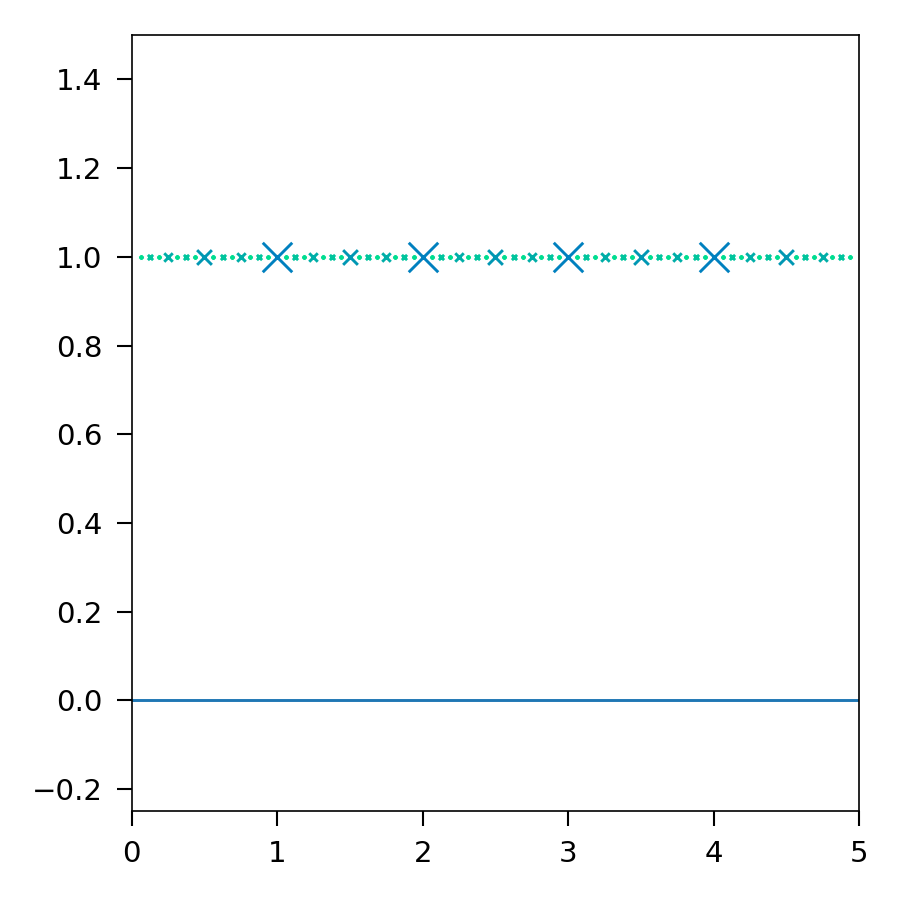
\includegraphics[]{Code/Rational.png}
	\caption{An illustration of the above indicator function, showing a few rationals that are multiples of negative powers of 2.}
\end{figure}

First, let's define the Riemann integral. The definition of the Riemann integral involves a few steps, and so it's going to take a little patience. The first step is defining a step function (no pun intended).

A function is called a step function if and only if there exists some finite sequence of points (which we can index by n and call $x_n$) such that the function is constant between any two adjacent points. So given the function with the graph;
\begin{figure}[H]
	\centering
	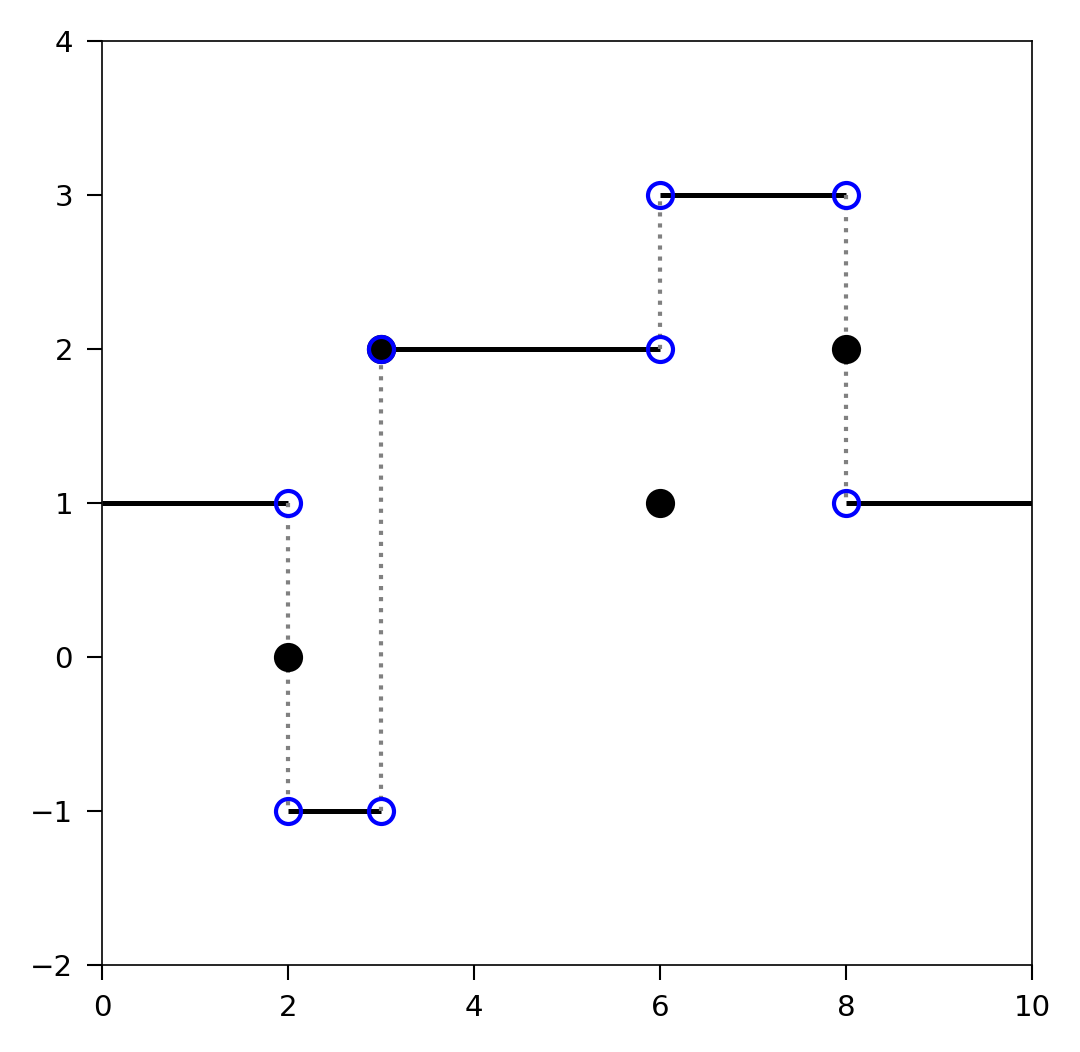
\includegraphics{Code/Step.png}
	\caption{A Step Function}
\end{figure}
the points \{0, 2, 3, 6, 8, 10\} are the finite sequence which make this a step function. Note two important facts;
\begin{itemize}
	\item We could have picked the points \{0, 1, 2, 3, 4, 5, 6, 7, 8, 9, 10\} to be our finite sequence, as the above function also happens to constant between any two adjacent integers. 
	\item It doesn't really matter what the function is {\em at} the points $x_n$, since we only care whether the function is constant {\em between} the points. In our graph, 2, 3, 6, and 8 are discontinues, but that doesn't matter since they're also in our sequence of points. 
\end{itemize}

The formal definition is as follows;
\begin{definition}{{(\bf\em Step Function\/})}
, $f: \ [a, b] \rightarrow \R$ is a step function if and only if there exists $n \in  \N$ and $a = x_0$
\end{definition}



